\chapter{Classificação de dados}
Para a realização da classificação de dados em padrões são necessárias as etapas de obtenção e organização dos dados, treinamento, que na metologia utilizada nesse trabalho corresponde a geração dos hiperplanos separadores através do MPLHS, e teste, onde é feita a classificação de um dado com padrão inicialmente desconhecido.
Todo o processo, desde a organização dos dados até a etapa de classificação, foi implementado utilizando a linguagem de programação Java. A implementação foi feita em módulos, organizados da seguinte forma: Módulo organizador de dados, Módulo de geração de classificadores, Módulo de classificação, Módulo validador. No módulo organizador de dados os conjuntos de dados são organizados em subgrupos, cada subgrupo contendo vetores de todos os padrões, essa organização é importante para a etapa de validação do método. No Módulo de geração de classificadores está implementado o MPLHS e são gerados os hiperplanos separadores. Os Módulos de classificação e validador são utilizados na etapa de teste, o primeiro realiza a classificação de um vetor em um dos padrões separados pelo hiperplano e o segundo realiza a validação do método de classificação de dados utilizando o método cross validation.

Na figura \ref{img:diagrama_modulos} estão representadas as etapas da metodologia utilizada para a classificação de dados em padrões.

\begin{center}
	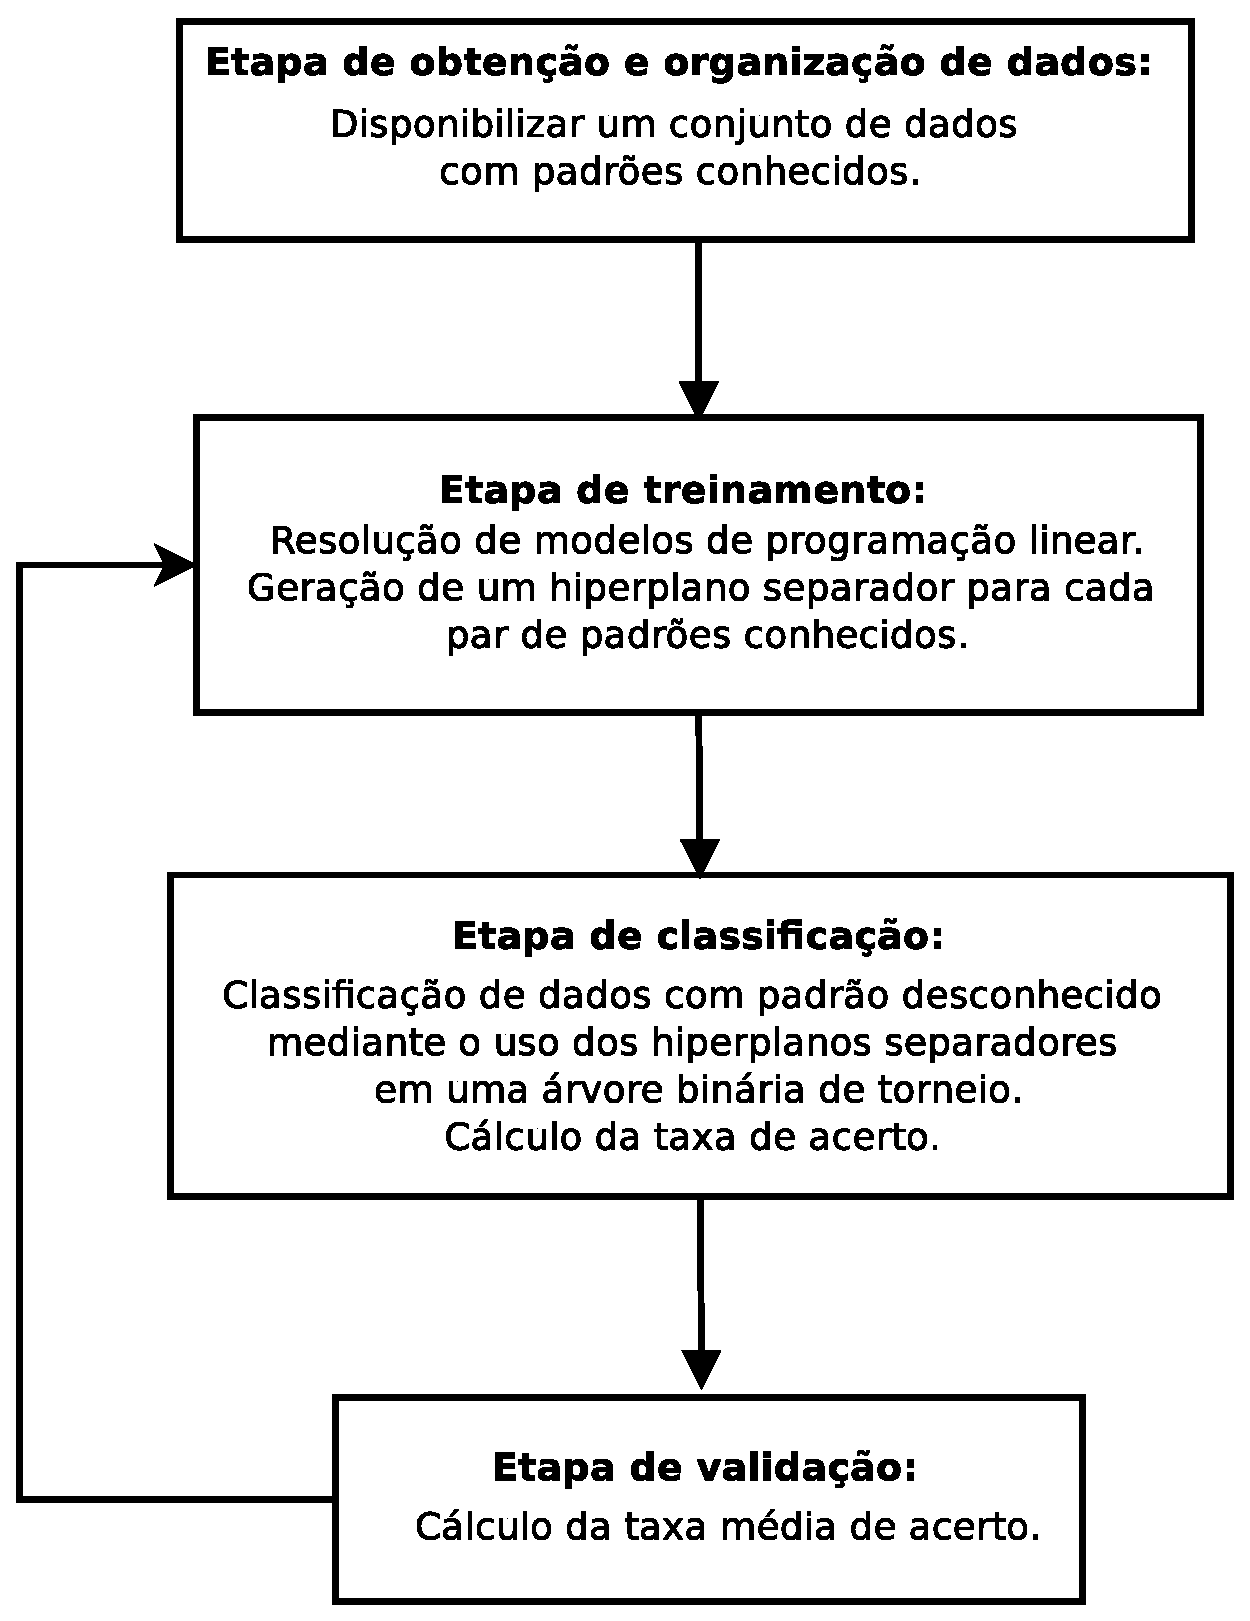
\includegraphics[scale=0.5]{graficos/Diagrama_etapas}
	\captionof{figure}{Diagrama das etapas da metodologia}
	\label{img:diagrama_modulos}
\end{center}

Primeiramente os dados foram obtidos já no formato de vetores de características ou  extraídos de imagens, e depois foram divididos em subgrupos. Em seguida, foram submetidos ao MPLHS, responsável por gerar os classificadores e por último vetores com padrão desconhecido foram classificados. As duas últimas etapas são repetidas a cada ciclo de teste, essas repetições são controladas pelo módulo validador. Nas seções seguintes essas etapas serão apresentadas de forma mais detalhada.

\section{Etapa de obtenção e organização de dados}
Nessa etapa inicial é obtido um conjunto de dados com um número de padrões \textit{p}, esse conjunto é composto por vetores contendo \textit{n} características. Para a classificação dos dados, o número \textit{p} de padrões deve ser previamente conhecido, assim como o número de vetores de características para cada padrão. 
A organização consiste em dividir o conjunto de dados em subconjuntos. A cada ciclo de treinamento e teste, alguns desses subconjuntos de dados são utilizados para treinamento enquanto um subconjunto será utilizados para teste. Cada vetor utilizado para teste será classificado em um dos \textit{p} padrões previamente conhecidos.

\section{Etapa de treinamento}
Na tarefa onde o objetivo é a separação de dois ou mais conjuntos de pontos, sendo que cada conjunto representa um padrão, busca-se um método para que essa separação seja obtida com resultado ótimo. Cada padrão é representado por de um conjunto de pontos e cada ponto é representado por um vetor de características.
Em \cite{Bennett92robustlinear} é proposto um MPLHS capaz de gerar um hiperplano, que separa dois conjuntos de pontos, minimizando a soma das médias das violações dos pontos que permaneceram do lado "errado" do hiperplano. Dessa forma o MPLHS é capaz de gerar um hiperplano separador para conjuntos de pontos linearmente separáveis e para conjuntos linearmente inseparáveis, o MPLHS gera o melhor hiperplano de forma que essa soma das médias calculada seja mínima. Na figura abaixo estão ilustrados os casos de dois conjuntos linearmente separáveis e dois conjuntos linearmente inseparáveis.
 
\begin{figure}[!h]
\centering
\subfigure[]{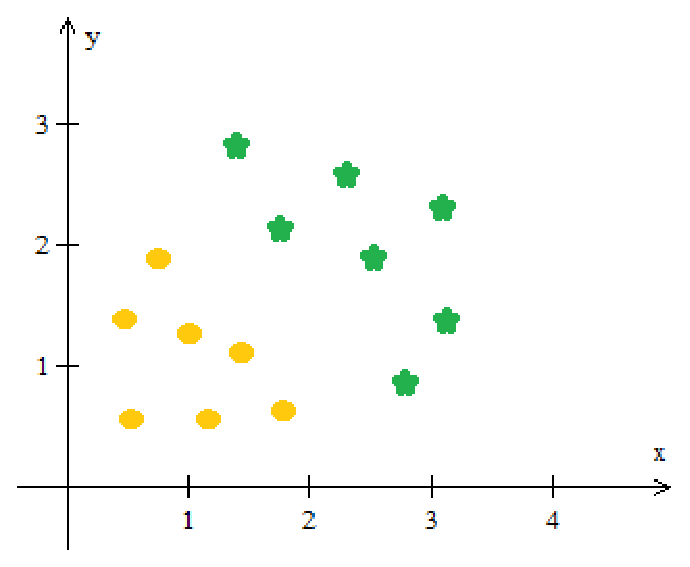
\includegraphics[scale=0.5]{graficos/linear_sepa}\label{fig1}}
\qquad
\subfigure[]{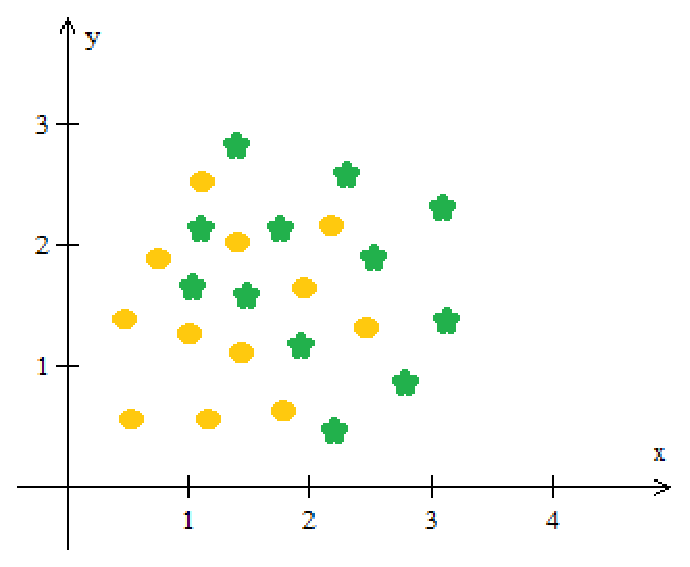
\includegraphics[scale=0.5]{graficos/linear_insepa}\label{fig2}}
\label{img:linear_sepa}
\caption{Conjuntos linearmente separáveis e linearmente inseparáveis}
\end{figure}

Em \ref{fig1} são apresentados dois conjuntos linearmente separáveis e em \ref{fig2} são apresentados dois conjuntos linearmente inseparáveis
É possível observar que na figura \ref{fig1} podem ser traçadas inúmeras retas separando os dois conjuntos de pontos. Já na figura \ref{fig2} o MPLHS de programação linear poderá definir a melhor reta possível para separar os pontos.

A proposta do MPLHS é separar dois conjuntos de pontos, porém também pode ser utilizado em problemas onde busca-se a separação de múltiplos padrões. O presente trabalho foca nessa última abordagem, em todos os testes realizados o número de conjuntos de pontos é igual ou maior que três.

\subsection{O modelo (MPLHS)}
Considerando dois conjuntos, no espaço n-dimensional $ R^{n} $, sendo o conjunto A representado pela matriz m x n, e o conjunto B representado pela matriz k x n. Contextualizando, k e m são as quantidades de pontos em cada conjunto, sendo que cada vetor de características é um ponto e n é a quantidade de características. O MPLHS calcula um hiperplano que procura separar os pontos dos dois conjuntos. De forma que os m pontos do conjunto A fiquem de um lado do hiperplano e os k pontos do conjunto B fiquem do outro lado do hiperplano. Nos casos em que os conjuntos não são separáveis, alguns pontos ficam localizados do lado "errado" do hiperplano. Na figura abaixo o MPLHS é apresentado. E a seguir é apresentado de forma mais detalhada.
\newpage
$$\min_{\omega ,\gamma ,y,z}\frac{e^{T}y}{m}+\frac{e^{T}z}{k}$$
$$s.a.\left\{\begin{matrix}-A\omega +e\gamma+e\leq y\\B\omega -e\gamma+e\leq  z\\ y\geq 0,y\geq 0\end{matrix}\right.$$

O MPLHS determina o hiperplano:
$$ x\omega = \gamma $$
Onde,  é $\omega$ o vetor normal ao hiperplano e $\gamma$ é um escalar. De forma que:
$$A\omega \geq e\gamma$$
e
$$B\omega \leq e\gamma$$
Onde e é um vetor de 1’s com dimensão m para o conjunto A e k para o conjunto B.
Para conjuntos linearmente separáveis torna-se fácil traçar um hiperplano separador, porém para conjuntos linearmente inseparáveis é necessária uma estratégia. Na busca pelo melhor hiperplano, o MPLHS gera dois hiperplanos limites somando ou subtraindo 1 unidade a equação do hiperplano separador:
$$A\omega \geq e\gamma + e$$
e
$$B\omega \leq e\gamma - e$$

De forma que o hiperplano separador fica localizado exatamente entre esses dois hiperplanos que formam uma faixa limite.
Nesse caso a estratégia utilizada é a minimização da soma das médias das violações dos pontos localizados do lado "errado" do hiperplano e também é considerada um violação o ponto que se localiza na faixa limite.
Detalhando o MPLHS de acordo com \citeonline{Eberson10LPseparaPontos}, considerando x como um vetor em $ R^{n} $, definimos:

$1.\ \ (x_{i})_{+} = \max_{i=1,2,...,n}{\left \{x_{i},0  \right \}}$

$2.\ \ \left \| x \right \|_{1} = \sum_{i=1}^{n}\left | x_{i} \right |$

Podemos escrever o problema de minimização com norma da seguinte forma:

$$\min_{\omega ,\gamma }\frac{1}{m}\left \| \left ( -A\omega + e\gamma  + e \right )_{+} \right \|_{1} + \frac{1}{k}\left \| \left ( B\omega - e\gamma + e  \right )_{+} \right \|_{1}$$

Seja $g:R^{n} \mapsto R^{m} , h:R^{n} \mapsto R^{k}$ e S um subconjunto de $R^{n}$ . Os problemas abaixo possuem soluções idênticas:

$$\min_{x\in S}\left \| g(x)_{+} \right \|_{1} + \left \| h(x)_{+} \right \|_{1}$$


$$\min_{x\in S} e^{t}y + e^{t}z\\$$
$$ s.a.\left\{\begin{matrix}y\geq g(x)\\ z\geq h(x)\\ y\geq 0, z\geq0\end{matrix}\right.$$

Como $g(x)_{+}\geq g(x)$ e $h(x)_{+}\geq h(x)$ podemos observar que os valores ótimos de y e z podem ser dados pelas igualdades $y=g(x)_{+}$ e $z=h(x)_{+}$.

A partir do problema de minimização temos o problema de programação linear equivalente:
\begin{eqnarray}
\min_{\omega ,\gamma ,y,z}\frac{e^{T}y}{m}+\frac{e^{T}z}{k} \label{eq3:obj1}\\
Sujeito\ a \nonumber\\
-A\omega +e\gamma+e\leq y\label{eq3:rest1}\\
B\omega -e\gamma+e\leq  z \label{eq3:rest2}\\ 
y\geq 0,y\geq 0 \label{eq3:rest3}
\end{eqnarray}

\underline{Dados do MPLHS}:
\begin{itemize}
\item{m}: quantidade de vetores de características correspondente ao primeiro padrão;
\item{k}: quantidade de vetores de características correspondente ao segundo padrão;
\item{A}: Matriz contendo o conjunto de vetores de caraterísticas do primeiro padrão;
\item{B}: Matriz contendo o conjunto de vetores de caraterísticas do segundo padrão;
\item{e}: vetor coluna unitário;
\end{itemize}

\underline{Variáveis do MPLHS}:
\begin{itemize}
\item{$\omega$}: coeficientes do hiperplano que separa os conjuntos de pontos dos dois padrões;
\item{$\gamma$}: constante do hiperplano que separa os conjuntos de pontos dos dois padrões;
\item{y}: vetor contendo o quanto um ponto do conjunto A violou o hiperplano limite;
\item{z}: vetor contendo o quanto um ponto do conjunto B violou o hiperplano limite;.
\end{itemize}

\underline{Formulação Matemática}:
A função objetivo \ref{eq3:obj1} procura minimizar a soma das médias das violações dos pontos de ambos conjuntos. A restrição \ref{eq3:rest1} exige que os pontos do conjunto A permaneçam do mesmo lado da reta fora da faixa limite definida pelos hiperplanos limite.  A restrição \ref{eq3:rest2} é análoga a restrição \ref{eq3:rest1} aplicada ao conjunto B. As equações em \ref{eq3:rest3} definem a natureza das variáveis do MPLHS, como sendo não negativas.

\subsection{Exemplo Ilustrativo do MPLHS}
Para ilustrar o MPLHS vamos considerar dois exemplos em $R^{2}$ \cite{Bennett92robustlinear} de forma que a ilustração gráfica fique mais facilmente compreensível.
\begin{itemize}
\item Exemplo1:
\end{itemize}

Considerando as matrizes a seguir:
$$A=\begin{bmatrix}1 & 1\\ 1 & 2\\ 1 & 3\\ 2 & 1\\ 2 & 2\\ 2 & 3\\ 2 & 4\\ 3 & 3\\ 3 & 4\end{bmatrix}
B=\begin{bmatrix}4 & 1\\ 4 & 2\\ 4 & 3\\ 5 & 2\\ 5 & 3\\ 5 & 4\\ 6 & 2\end{bmatrix}$$

Nesse caso, temos: m = 9 (quantidade de pontos da matriz A) e k = 7 (quantidade de pontos da matriz B).  Resolvendo o MPLHS temos:
\begin{itemize}
\item[$\ast$] Valor da função objetivo = 0
\item[$\ast$] $\omega$ = [-2  0]
\item[$\ast$] $\gamma$ = -7
\item[$\ast$] y = [0 0 0 0 0 0 0 0 0]
\item[$\ast$] z = [0 0 0 0 0 0 0]
\end{itemize}
Como o valor da função objetivo depende dos vetores y e z, podemos notar que o valor 0 indica que os conjuntos A e B são linearmente separáveis. A seguir é apresentada a representação gráfica dos pontos e das retas geradas pelo MPLHS.

\begin{center}
	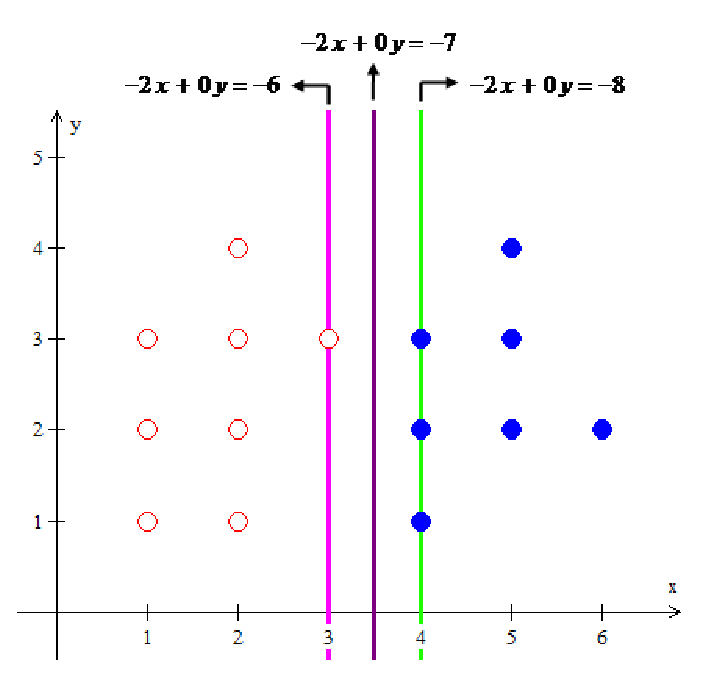
\includegraphics[scale=0.5]{graficos/exemplo2}
	\captionof{figure}{Representação ilustrativa do exemplo 1}
	\label{img:ex1}
\end{center}

A partir da representação gráfica podemos perceber que a reta separadora $-2x + 0y = -7$ se localizou exatamente entre os dois conjuntos com o auxílio das duas retas: $-2x + 0y = -6$ e $-2x + 0y = -8$.

\begin{itemize}
\item Exemplo2:
\end{itemize}
Vamos  considerar agora as matrizes:
$$A=\begin{bmatrix}3 & 4\\ 4.3 & 4.5\\ 4.5 & 2\\ 3 & 5.5\end{bmatrix}
B=\begin{bmatrix}4 & 2\\ 4.5 & 3.5\\ 5 & 3\end{bmatrix}$$

Neste exemplo temos: m = 4 e k = 3. De acordo com o MPLHS, temos os seguintes valores:
\begin{itemize}
\item[$\ast$] Valor da função objetivo = 0.92
\item[$\ast$] $\omega$ = [-0.91  0.91]
\item[$\ast$] $\gamma$ = -0.82
\item[$\ast$] y = [0 0 2.46 0]
\item[$\ast$] z = [0 0.91 0]
\end{itemize}

Com o valor da função objetivo diferente de zero, temos dois conjuntos linearmente inseparáveis, como ilustrado na figura a seguir. Nesse caso, a reta separa os pontos de ambos os conjuntos minimizando a soma das médias das violações.

\begin{center}
	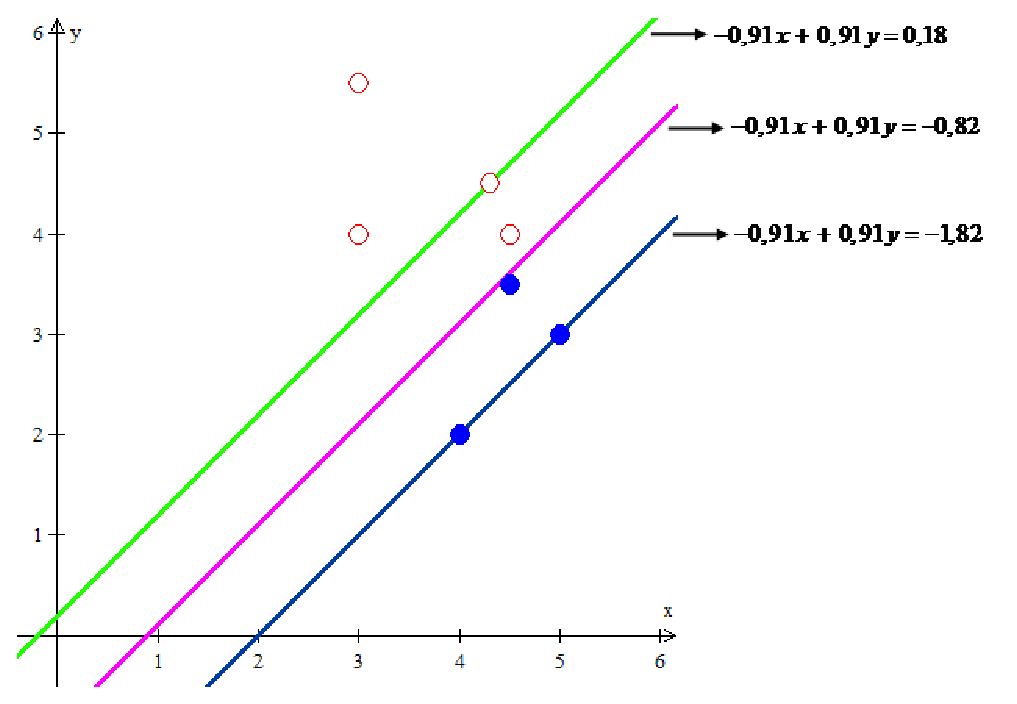
\includegraphics[scale=0.5]{graficos/exemplo1}
	\captionof{figure}{Representação ilustrativa do exemplo 2}
	\label{img:ex2}
\end{center}

Nesse exemplo notamos que o valor 2.46 no vetor y é referente ao ponto do conjunto A que está localizado do lado "errado" da reta. E o valor 0.91 é referente ao ponto do conjunto B que está localizado mais próximo à reta separadora, apesar do ponto estar localizado do ponto correto da reta ele está localizado acima da reta limite $-0.91x + 0.91y = -1.82$. Concluindo que, quando um ponto está localizado do lado "correto" do hiperplano ou em cima de um dos hiperplanos limites, seu valor correspondente no vetor y ou z é nulo. Mas se um ponto está localizado do lado "errado" do hiperplano ou dentro da faixa formado pelos hiperplanos limites, seu valor correspondente no vetor y ou z é positivo.

\subsection{Geração de hiperplanos separadores}
Na etapa de treinamento, os padrões são agrupados em pares e dessa forma são submetidos ao MPLHS, já que o modelo gera um hiperplano que separa dois padrões. Dessa forma para um conjunto de dados com N padrões, a quantidade de pares formados é dada pela fórmula:
$$ C_{N}^{2}=\frac{N!}{2\times (N-2)!)} $$

A etapa de treinamento consiste em gerar um hiperplano para cada par formado. No caso de um conjunto de dados constituído por 3 padrões, são gerados 3 hiperplanos separadores, da seguinte forma:

\begin{center}
	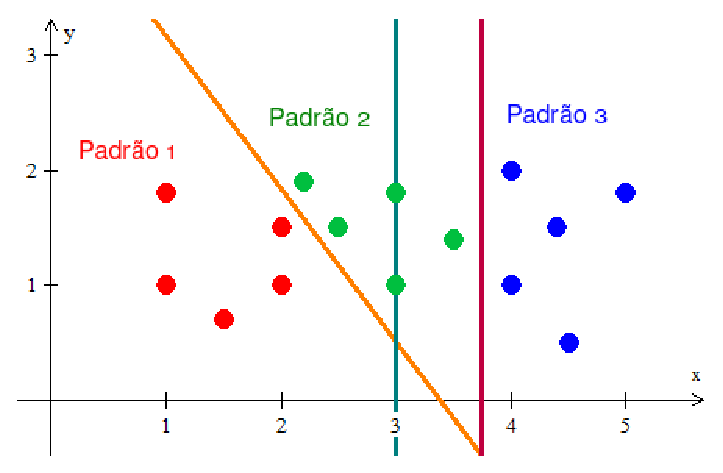
\includegraphics[scale=0.5]{graficos/class123}
	\captionof{figure}{Hiperplanos para um conjunto de dados com 3 padrões}
	\label{img:classificadores}
\end{center}

Na figura \ref{img:classificadores} é apresentada uma visão geral dos 3 conjuntos de pontos (padrões) e dos 3 hiperplanos separadores. A seguir os hiperplanos são apresentados separadamente, o MPLHS é resolvido 3 vezes, uma para cada par de padrões e cada resolução o modelo calcula um hiperplano separador para o par.
\newpage 
\begin{figure}[!h]
\centering
\subfigure[Classificador dos padrões 1 e 2]{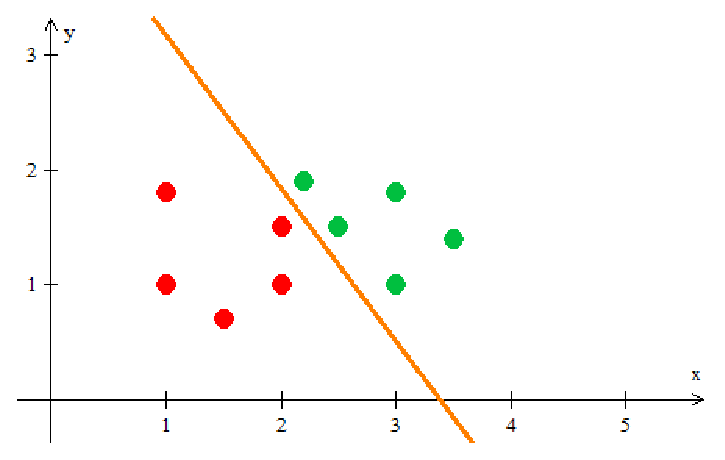
\includegraphics[scale=0.5]{graficos/class1e2}\label{fig1_ls}}
\qquad
\subfigure[Classificador dos padrões 1 e 3]{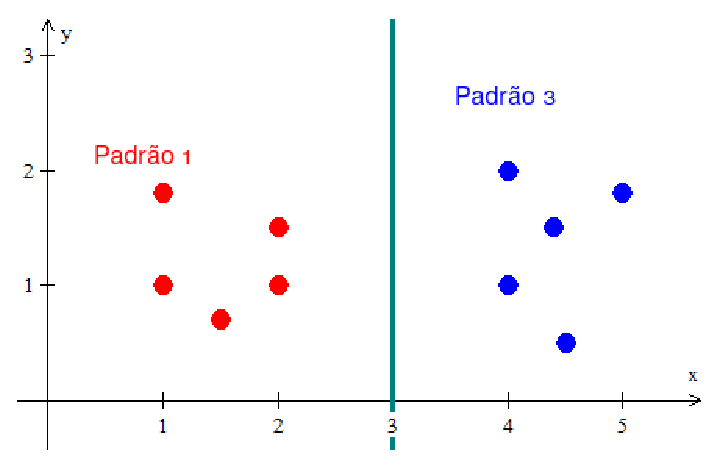
\includegraphics[scale=0.5]{graficos/class1e3}\label{fig2_ls}}
\qquad
\subfigure[Classificador dos padrões 2 e 3]{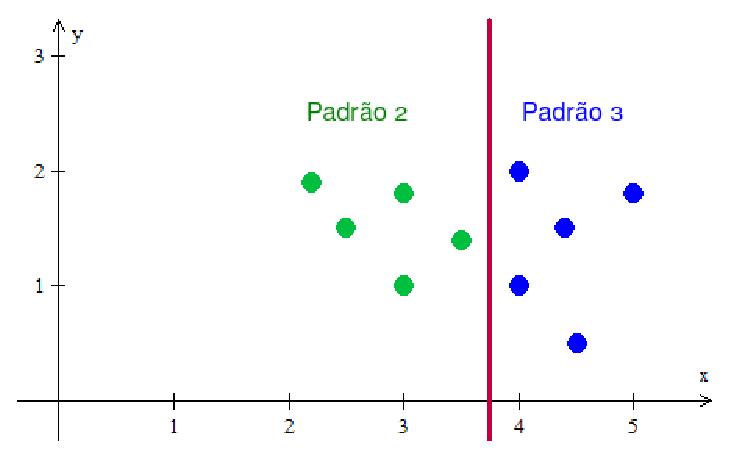
\includegraphics[scale=0.5]{graficos/class2e3}\label{fig3_ls}}
\label{img:class_separados}
\caption{Hiperplanos para um conjunto de dados com os 3 padrões organizados em pares}
\end{figure}

Na figura \ref{fig1_ls}, os padrões 1 e 2 foram submetidos ao MPLHS, e o hiperplano separador foi gerado para esses dois padrões. O mesmo ocorre nas figuras \ref{fig2_ls} e \ref{fig3_ls}, para cada para de padrões submetidos ao MPLHS, um hiperplano separador foi gerado.

O processo de treinamento corresponde ao módulo de geração de classificadores. Esse módulo foi implementado na linguagem de programação JAVA, utilizada como interface com o software CPLEX da IBM. O MPLHS é resolvido utilizando o método simplex revisado e toda etapa de resolução é feita pelo software CPLEX. A implementação desse módulo encontra-se no Apêndice A.

\section{Etapa de classificação} 
Após a geração dos classificadores utilizando o MPLHS, é necessário um segundo procedimento onde ocorra de fato a classificação de um vetor com padrão inicialmente desconhecido. Nessa etapa de classificação foi implementada uma estrutura de árvore binária de torneio. Em seus trabalhos, \citeonline{Feng} e \citeonline{Guo} utilizaram essa mesma estrutura na etapa de classificação após a utilização do MPLHS para gerar os classificadores.
No processo de teste, um vetor de características é submetido a estrutura de árvore binária de torneio e classificado em um dos \textit{p} padrões do conjunto de dados.
A cada teste uma árvore binária de torneio é construída a partir dos nós folhas e um vetor de características é classificado. Na estrutura de árvore binária de torneio os padrões são confrontados aos pares, o nó pai é obtido com base no hiperplano que separa os padrões que estão no nós filhos.%e o hiperplano que separa os dois padrões do par é utilizado para verificar de qual lado do hiperplano o vetor teste se localiza, o padrão que estiver do mesmo lado do hiperplano que o vetor que está sendo classificado é elevado ao nível superior da árvore.
A seguir é apresentada uma figura para ilustrar o mecanismo da árvore de torneio.

\begin{center}
	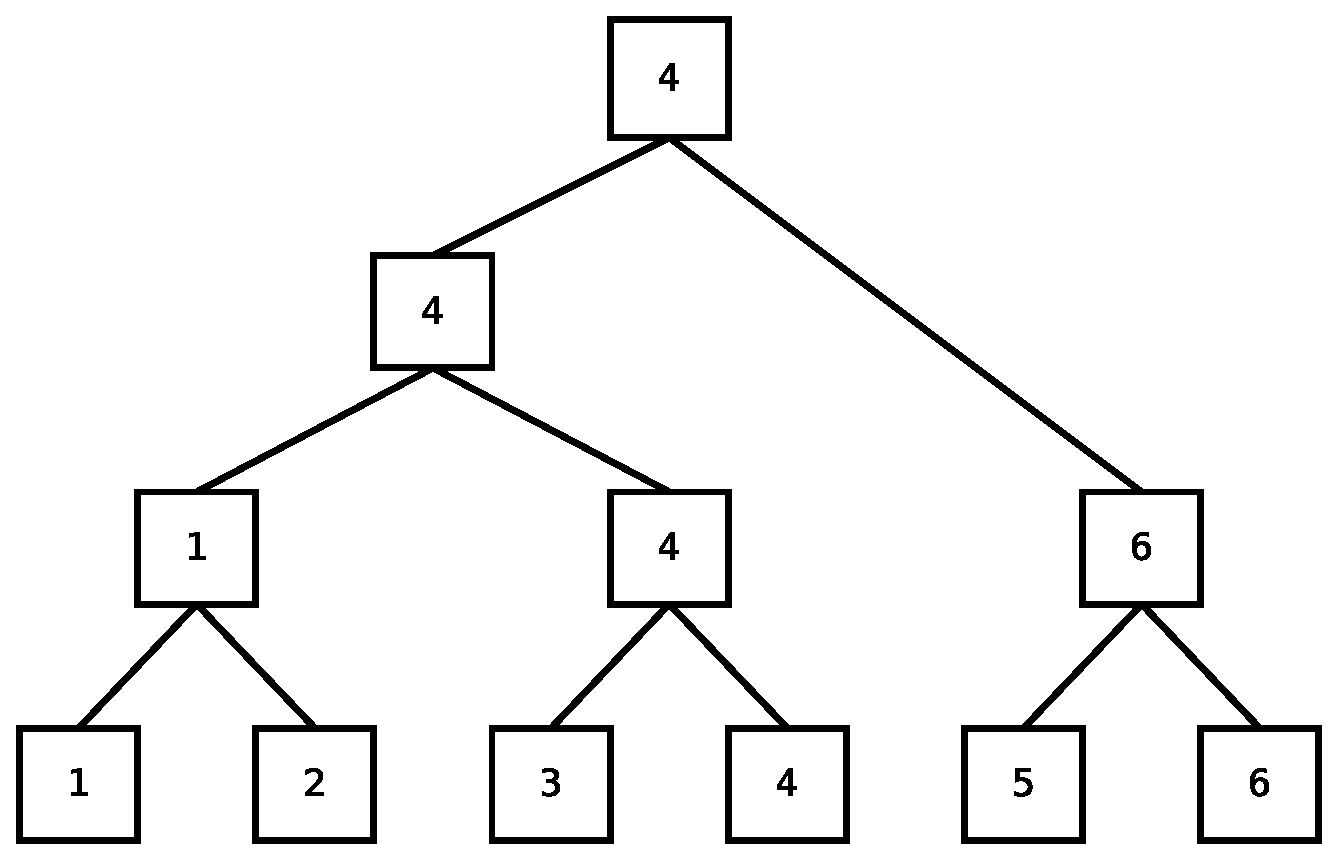
\includegraphics[scale=0.4]{graficos/ArvTorneio1}
	\captionof{figure}{Ilustração de uma árvore de torneio com 6 padrões}
	\label{img:ArvTorneio1}
\end{center}

Por analogia podemos pensar na árvore como a estrutura utilizada em um torneio esportivo e nos padrões como os times do torneio, os times devem se confrontar até que ao final saia o vencedor. Da mesma forma, analisamos os padrões até que ao final se obtenha o padrão ao qual o vetor pertence.
Na árvore da figura \ref{img:ArvTorneio1}, consideramos 6 padrões e o conjunto desconhecido pertencendo ao padrão 4. A quantidade de nós folhas deve ser a quantidade de padrões e a formação dos pares é arbitrária. Analisando o primeiro par, deve ser analisado em qual dos dois padrões o conjunto desconhecido mais se encaixa, ou seja, deve ser analisado de qual lado do hiperplano (gerado pelo MPLHS quando foram submetidos os padrões 1 e 2) o conjunto desconhecido se encontra. Na figura exemplo, o ponto representado pelo vetor de características ficou localizado do mesmo lado do hiperplano que os pontos do padrão 1, por isso esse padrão continuou no próximo nível da árvore e o padrão 2 foi excluído. Esse procedimento ocorre por analogia em todos os pares, até que ao final, quando analisados os padrões 4 e 6, foi definido que o vetor pertence ao padrão 4.

\subsection{Classificação com base em um hiperplano}
Dado um vetor x de características, para determinar a qual padrão esse vetor pertence deve ser analisado de qual lado do hiperplano o ponto dado pelo vetor, se localiza, considerando que 
\\Se $ \begin{bmatrix}
\omega _{1} & ... & \omega _{n} 
\end{bmatrix}
\begin{bmatrix}
x_{1}
\\ 
.
\\
. 
\\
. 
\\
x_{n}
\end{bmatrix}
\geq \gamma $, x pertence ao padrão A;

Se $ \begin{bmatrix}
\omega _{1} & ... & \omega _{n} 
\end{bmatrix}
\begin{bmatrix}
x_{1}
\\ 
.
\\
. 
\\
. 
\\
x_{n}
\end{bmatrix}
\leq  \gamma $, x pertence ao padrão B.

Considerando o seguinte hiperplano em $R^{4}$:
$\omega$ = [1.21  8.0  -6.4  -19.2]
$\gamma$ = -33.6

E o vetor $x$ = [6.7  3.0  5.2  2.3], temos:

$ \begin{bmatrix}
1.21 & 8.0 & -6.4 & -19.2 
\end{bmatrix}
\begin{bmatrix}
6.7
\\ 
3.0
\\
5.2 
\\
2.3 
\end{bmatrix}
\leq  -33.6 $ 

Nesse caso o ponto representado pelo vetor x permaneceu do mesmo lado do hiperplano que os pontos do padrão B, sendo assim o vetor de características x é reconhecido como pertencente ao padrão B. 

\subsection{Classificação utilizando a estrutura da árvore binária de torneio}
Para o caso apresentado anteriormente foram considerados apenas dois padrões, porém em um problema que considera três ou mais padrões, é necessária uma lógica para que seja realizada classificação do dado em um padrão entre os \textit{p} padrões existentes. Nesse caso é utilizada a árvore binária de torneio.
Considerando um exemplo com três padrões (A, B e C), e os seguintes hiperplanos em $R^{4}$:
\begin{itemize}
\item Hiperplano separador dos padrões A e B
\subitem $\omega$ = [1.14  0.0  0.0  -7.86]
\subitem $\gamma$ = 0.0
\item Hiperplano separador dos padrões A e C
\subitem $\omega$ = [0.62  0.0  -1.03  0.0]
\subitem $\gamma$ = 0.0
\item Hiperplano separador dos padrões B e C
\subitem $\omega$ = [1.21  8.0  -6.4  -19.2]
\subitem $\gamma$ = -33.6
\end{itemize}

Para determinar a qual dos três padrões pertence o vetor $x = [4.8\ \ 3.0\ \ 1.4\ \ 0.3]$, a árvore binária de torneio é montada dinamicamente iniciando pelo nível de maior profundidade, nesse exemplo iniciamos com os padrões A e B.

\begin{center}
	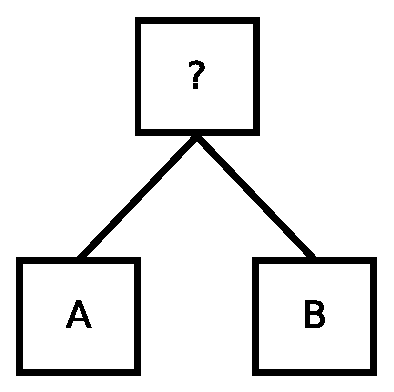
\includegraphics[scale=0.4]{graficos/arvore_nivel1}
	\captionof{figure}{Nós folhas no nível de maior profundidade}
	\label{img:Arv_nivel1}
\end{center}

Iniciando a classificação do vetor x analisando os padrões A e B como ilustrado pela figura \ref{img:Arv_nivel1}, deve ser verificado de qual lado do hiperplano separador dos padrões A e B o ponto representado pelo vetor x permanecerá
$ \begin{bmatrix}
4.8 & 3.0 & 1.4 & 0.3 
\end{bmatrix}
\begin{bmatrix}
1.14
\\ 
0.0
\\
0.0 
\\
-7.86 
\end{bmatrix}
\geq  0.0 $ 

Nessa primeira análise, o ponto representado pelo vetor x ficou localizado do mesmo lado do hiperplano que os pontos do padrão A. Então o padrão A é elevado ao próximo nível da árvore, como ilustrado na figura a seguir.

\begin{center}
	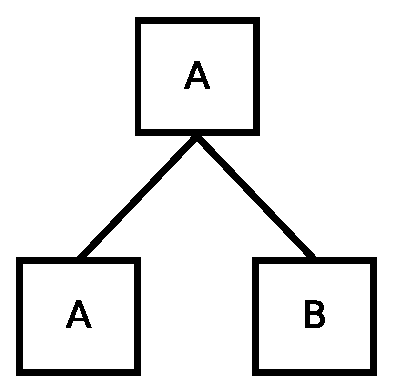
\includegraphics[scale=0.4]{graficos/arvore_nivel2}
	\captionof{figure}{Padrão A é elevado ao próximo nível da árvore}
	\label{img:Arv_nivel2}
\end{center}

Resta ainda analisar o padrão C.

\begin{center}
	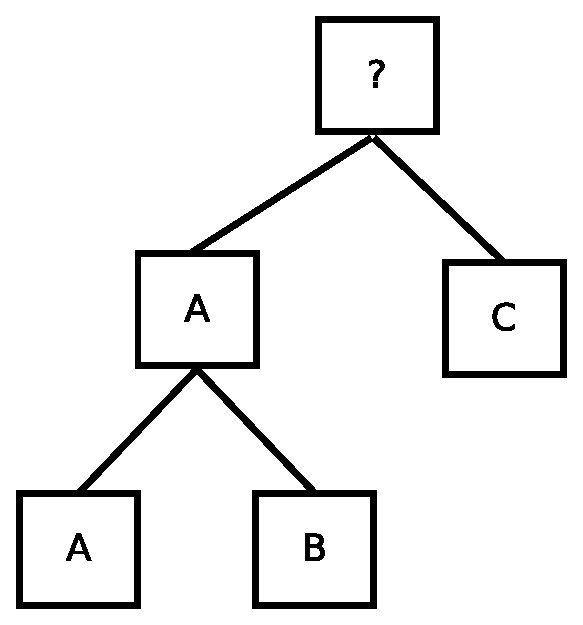
\includegraphics[scale=0.4]{graficos/arvore_nivel3}
	\captionof{figure}{Segundo nível da árvore}
	\label{img:Arv_nivel3}
\end{center}

Como mostrado na figura \ref{img:Arv_nivel3}, é feita a análise utilizando o hiperplano separador dos padrões A e C.
$ \begin{bmatrix}
4.8 & 3.0 & 1.4 & 0.3 
\end{bmatrix}
\begin{bmatrix}
0.62
\\ 
0.0
\\
-1.03
\\
0.0 
\end{bmatrix}
\geq  -33.6 $ 

Analisando o hiperplano separador dos padrões A e C é determinado que o ponto representado pelo vetor x ficou localizado do mesmo lado que os pontos do padrão A. Como todos os padrões (A, B e C) já foram analisados e a árvore foi completada, então, finalmente, o vetor x é reconhecido como pertencente ao padrão A.

\begin{center}
	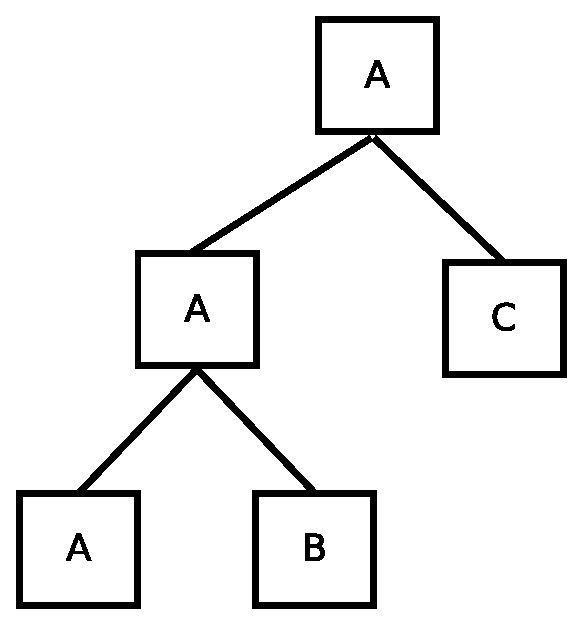
\includegraphics[scale=0.4]{graficos/arvore_completa}
	\captionof{figure}{Árvore completa}
	\label{img:Arv_completa}
\end{center}

A árvore completa é mostrada na figura \ref{img:Arv_completa}, após analisar todos os padrões, e o nó raiz da árvore ser preenchido, a etapa de classificação é completada, e o vetor com padrão inicialmente desconhecido é classificado como pertencente ao padrão que está no nó raiz da árvore.

\section{Etapa de validação}
Para testar a metodologia adotada neste trabalho para a classificação de dados, foi utilizado o método \textit{k-fold cross validation} \cite{Kohavi95Cross} \cite{Baldisserotto05Validacao}. Através dos resultados desse método é possível analisar a acurácia da metodologia de classificação, ou seja, a capacidade de classificar um dado com o seu padrão correto.
Entre os três métodos de validação apresentados no referencial teórico: \textit{Handout}, \textit{cross validation} e \textit{Leave One Out}. O método \textit{cross validation} foi escolhido como melhor opção já que os teste são feitos com conjuntos de dados com tamanhos variados. Para conjuntos de dados muito grandes o método \textit{leave one out} se tornaria computacionalmente custoso e o método \textit{handout} poderia ter seu resultado comprometido dependendo dos parâmetros escolhidos na separação de dados para teste e de dados para validação. Além disso, o método \textit{cross validation} é de fácil implementação e permite a utilização de todos os dados na etapa de teste e treinamento.
Na figura abaixo o método \textit{k-fold cross validation} é ilustrado com o parâmetro 5 \textit{fold}, apesar desse parâmetro não ter sido utilizado em nenhum teste, foi utilizado para um facilitar a ilustração. 
\begin{center}
	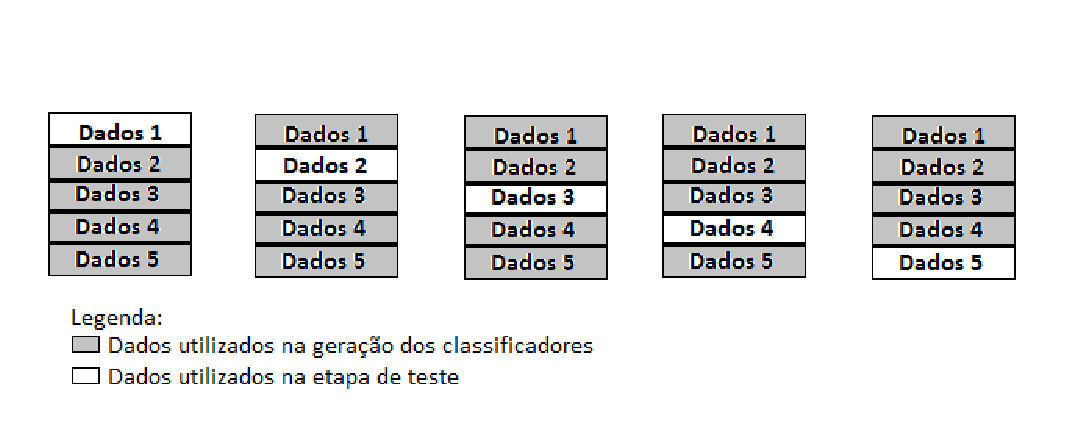
\includegraphics[scale=1.0]{graficos/cross_validation}
	\captionof{figure}{Mecanismo do método de validação 5- \it{fold cross validation}}
	\label{img:cross_validation}
\end{center}

Na ilustração o conjunto de dados é dividido em 5 subconjuntos e consequentemente são realizados 5 ciclos de treinamento e testes. A cada etapa 4 subconjuntos são utilizados para treinamento e um subconjunto diferente é utilizado para teste. 

A metodologia \textit{k-fold cross validation} foi implementada na linguagem de programação Java. Os dados são organizados em k arquivos (subconjuntos) e são realizados k ciclos de treinamento e teste. A implementação seleciona os arquivos para treinamento e o arquivo para teste, na etapa de teste de cada ciclo, todos os vetores do arquivo de teste são classificados. A cada ciclo de treinamento e teste a porcentagem de acerto de classificação é calculada da seguinte forma:

$$A = \frac{acertos}{total}\times 100$$

Onde total é a quantidade de vetores para classificação submetidos a cada ciclo de teste. E acertos é a quantidade de vetores que foram classificados corretamente.
Ao final dos k ciclos de treinamento e teste, é calculada a média das porcentagens de acerto obtidas a cada ciclo
